\documentclass[tikz,border=8pt]{standalone}
\usepackage{amsmath}
\usetikzlibrary{arrows.meta}
\begin{document}
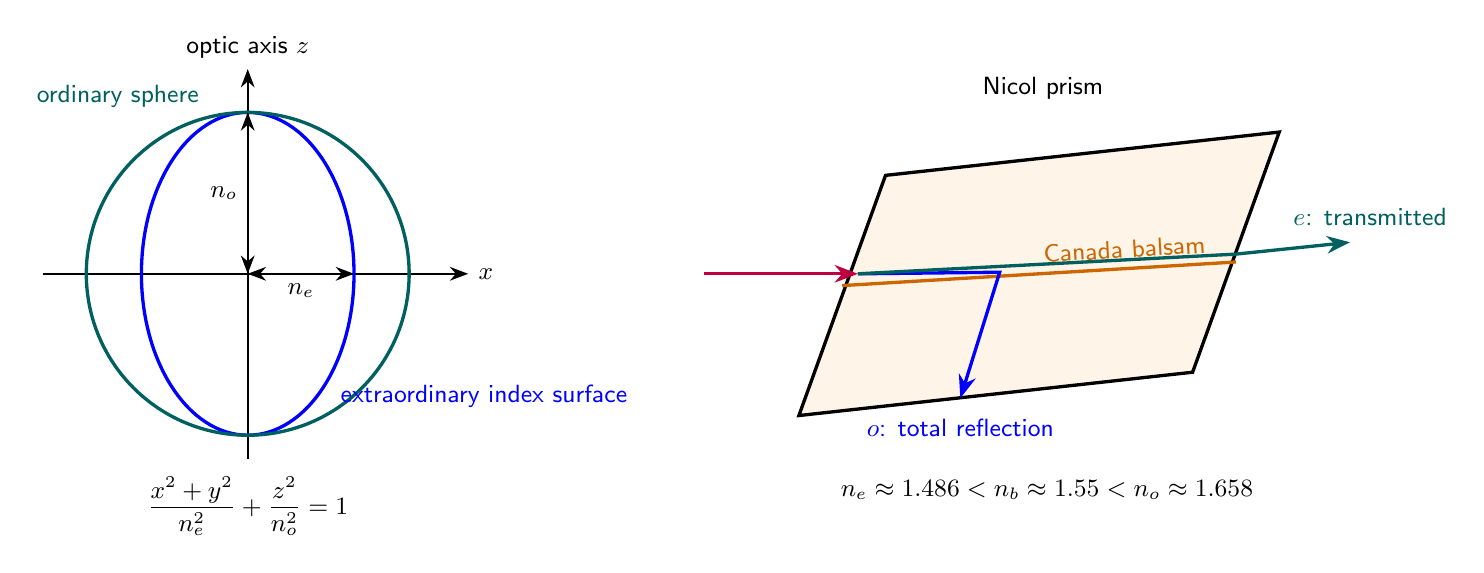
\begin{tikzpicture}[font=\sffamily\small,>=Stealth,thick]
  \begin{scope}
    \draw[->] (-2.6,0)--(2.8,0) node[right] {$x$};
    \draw[->] (0,-2.35)--(0,2.6) node[above] {optic axis $z$};
    \draw[blue,very thick] (0,0) ellipse (1.35 and 2.05);
    \draw[teal!75!black,very thick] (0,0) circle (2.05);
    \draw[<->] (0,0)--(1.35,0) node[midway,below] {$n_e$};
    \draw[<->] (0,0)--(0,2.05) node[midway,left] {$n_o$};
    \node[teal!75!black] at (-1.65,2.25) {ordinary sphere};
    \node[blue,anchor=west] at (1.05,-1.55) {extraordinary index surface};
    \node[align=center] at (0,-2.95)
      {$\displaystyle \frac{x^2+y^2}{n_e^2}+\frac{z^2}{n_o^2}=1$};
  \end{scope}
  \begin{scope}[xshift=7cm]
    \fill[orange!9] (0,-1.8)--(5,-1.25)--(6.1,1.8)--(1.1,1.25)--cycle;
    \draw[very thick] (0,-1.8)--(5,-1.25)--(6.1,1.8)--(1.1,1.25)--cycle;
    \draw[very thick,orange!80!black] (.55,-.15)--(5.55,.15)
      node[pos=.72,above,sloped] {Canada balsam};
    \draw[->,purple,very thick] (-1.2,0)--(.75,0);
    \draw[->,blue,very thick] (.75,0)--(2.55,.02)--(2.05,-1.58);
    \node[blue,anchor=north] at (2.05,-1.72) {$o$: total reflection};
    \draw[->,teal!75!black,very thick] (.75,0)--(5.55,.25)--(7,.4);
    \node[teal!75!black,anchor=west] at (6.15,.72) {$e$: transmitted};
    \node at (3.1,2.35) {Nicol prism};
    \node[align=center] at (3.15,-2.75)
      {$n_e\approx1.486<n_b\approx1.55<n_o\approx1.658$};
  \end{scope}
\end{tikzpicture}
\end{document}
